\chapter{麦克斯韦方程组}\label{ch:b2:maxwell-equations}

1865 年，詹姆斯·克拉克·麦克斯韦写下了
库仑、安培和法拉第逐一发现的定律，
并在安培定律中添加了一项
当时尚无实验要求的项，
并发现他的方程允许一种以某一速率传播的波，
该速率可由电磁学的常数算出——即光速。
电学、磁学与光学原为同一门学科。本科一年级分册以面积分和回路积分的形式叙述这些定律；
本章则将它们写成四个\emph{局域}方程，在每一点、每一时刻都成立，
并引入使这种写法成为可能的矢量算符，
由此导出第一批结论：\omterm{thm:b2:maxwell-equations:maxwell}{位移电流}、势、
场在界面上的行为，
以及本科一年级分册中电路可精确适用的近似条件。

\begin{omfigure}
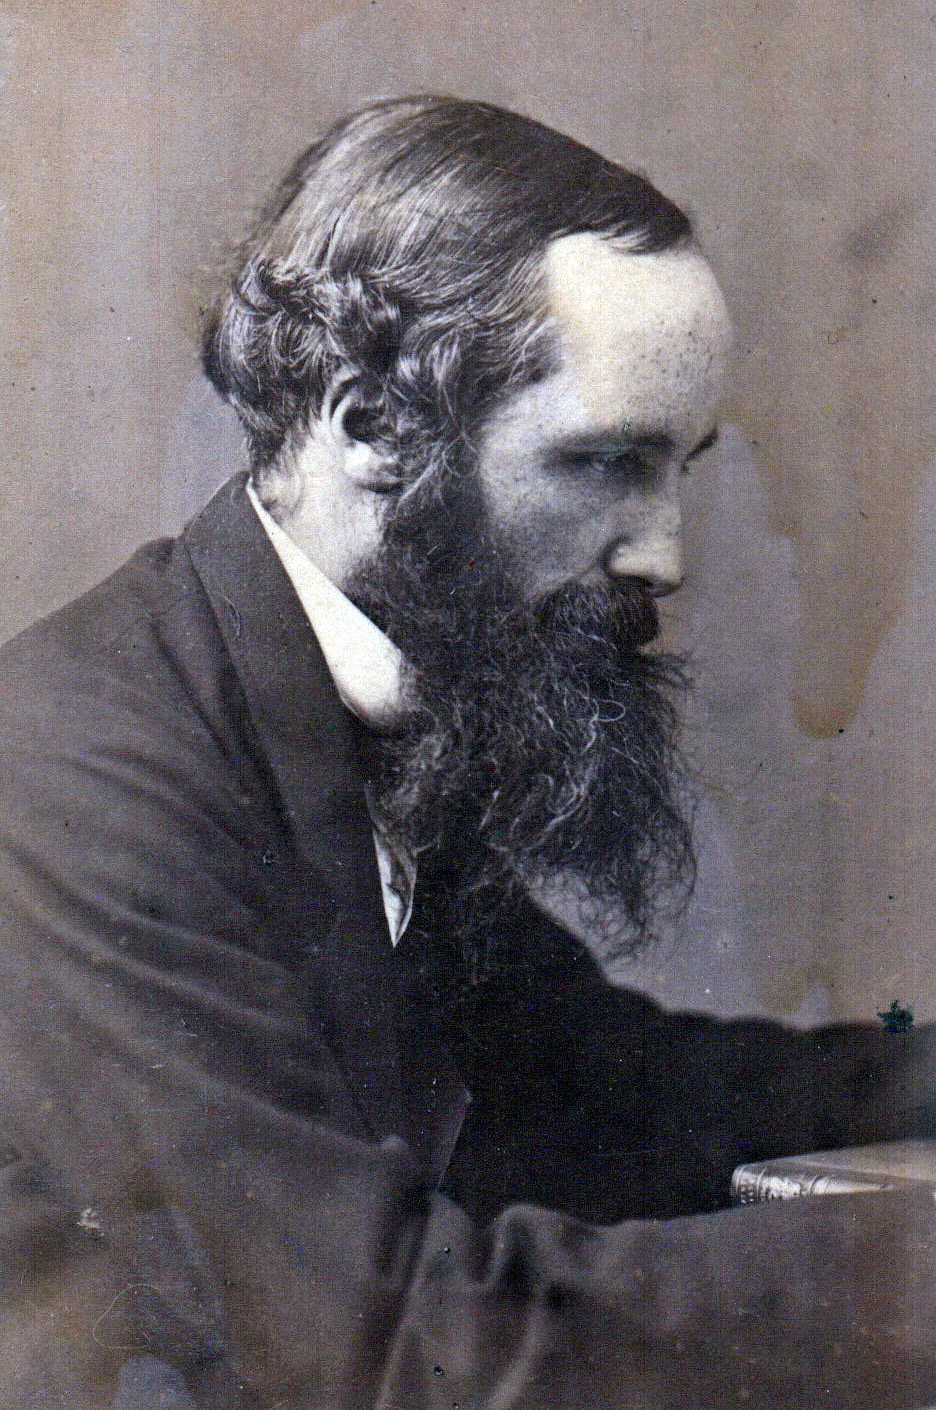
\includegraphics[width=0.3\linewidth]{images/book4/maxwell-profile.jpg}

{\small 詹姆斯·克拉克·麦克斯韦（1831--1879），写出了本章的四个方程，并从中读出了以光速传播的电磁波的存在。}
\end{omfigure}

\section{矢量算符}

\begin{definition}[梯度、散度、旋度、拉普拉斯算子]\label{def:b2:maxwell-equations:operators}
\index{梯度}\index{散度}\index{旋度}\index{拉普拉斯算子}\index{纳布拉算子}
设 $f$ 为标量场，$\vect A$ 为矢量场，在直角坐标系中，
记符号矢量 $\vect\nabla = (\partial_x, \partial_y,
\partial_z)$：
\begin{align*}
\operatorname{\vect{grad}}f &= \vect\nabla f = (\partial_xf,\ \partial_yf,\ \partial_zf) ,\\
\operatorname{div}\vect A &= \vect\nabla\cdot\vect A = \partial_xA_x + \partial_yA_y + \partial_zA_z ,\\
\operatorname{\vect{curl}}\vect A &= \vect\nabla\wedge\vect A = (\partial_yA_z - \partial_zA_y,\ \partial_zA_x - \partial_xA_z,\ \partial_xA_y - \partial_yA_x) ,\\
\Delta f &= \operatorname{div}\operatorname{\vect{grad}}f = \partial_x^2f + \partial_y^2f + \partial_z^2f ,
\end{align*}
而 $\Delta\vect A$ 为对各直角分量取拉普拉斯算子。
这些算符的意义与坐标选取无关：$\operatorname{\vect{grad}}f
\cdot\dd\vect l = \dd f$ 为 $f$ 沿 $\dd\vect l$ 的变化量；$\operatorname{div}
\vect A$ 为 $\vect A$ 穿过小体积表面的向外通量，
每单位体积；$\operatorname{\vect{curl}}\vect A\cdot\vect n$ 为
$\vect A$ 绕法向为 $\vect n$ 的小回路的环量，
每单位面积。
\end{definition}

\begin{theorem}[散度定理与斯托克斯定理]\label{thm:b2:maxwell-equations:theorems}
\index{散度定理}\index{奥斯特罗格拉茨基定理}\index{斯托克斯定理}
设闭曲面 $\Sigma$ 围成体积 $V$，
有向闭曲线 $C$ 张成曲面 $S$（法向 $\vect n$ 由
右手定则给出），则
\[
\iint_\Sigma\vect A\cdot\vect n\,\dd S = \iiint_V\operatorname{div}\vect A\,\dd\tau ,
\qquad
\oint_C\vect A\cdot\dd\vect l = \iint_S\operatorname{\vect{curl}}\vect A\cdot\vect n\,\dd S .
\]
\end{theorem}
\admitted

\begin{remark}[承认的内容及其可信之处]\label{rem:b2:maxwell-equations:whyadmitted}
两个定理均在本科三年级数学分册中证明；本科二年级数学分册只
讲到它们的平面形式（格林–黎曼公式）以及多重积分。然而，
其内容正是我们在
\cref{ch:b2:fluid-kinematics}中所用的：将体积划分为
小长方体（曲面则划分为小回路）——内部各面上的通量
（内部各棱上的环量）两两相消，只剩下边界部分。
由定义可直接得出两个恒等式，
并被经常使用：
$\operatorname{\vect{curl}}\operatorname{\vect{grad}}f = \vect 0$，
$\operatorname{div}\operatorname{\vect{curl}}\vect A = 0$，以及
$\operatorname{\vect{curl}}\operatorname{\vect{curl}}\vect A = \operatorname{\vect{grad}}
\operatorname{div}\vect A - \Delta\vect A$。对具有对称性的场，
常用公式为：对径向场 $A_r(r)\vect e_r$，$\operatorname{div}
= \frac1{r^2}\partial_r(r^2A_r)$（球坐标）或 $\frac1r\partial_r(rA_r)$
（柱坐标）；对绕轴的方位场 $A_\theta(r)\vect e_\theta$，
$(\operatorname{\vect{curl}})_z = \frac1r\partial_r(rA_\theta)$；对 $f(r)$，
$\Delta f = \frac1{r^2}\partial_r(r^2\partial_rf) = \frac1r\partial_r^2(rf)$（球坐标），
$\frac1r\partial_r(r\partial_rf)$（柱坐标）。
\end{remark}

\begin{omfigure}
\begin{tikzpicture}[font=\small, x=1cm, y=1cm, >=Stealth]
  \begin{scope}
    \draw[thick, fill=omDef!10] (0,0) rectangle (1.8,1.4);
    \draw[thick] (0,1.4) -- (0.5,1.85) -- (2.3,1.85) -- (1.8,1.4);
    \draw[thick] (1.8,0) -- (2.3,0.45) -- (2.3,1.85);
    \draw[omThm, thick, ->] (-0.9,0.7) -- (-0.1,0.7);
    \draw[omThm, thick, ->] (1.9,0.7) -- (3.0,0.7);
    \draw[omThm, thick, ->] (0.9,-0.8) -- (0.9,-0.1);
    \draw[omThm, thick, ->] (1.1,1.9) -- (1.1,2.7);
    \node[font=\footnotesize] at (1.0,-1.35) {$\operatorname{div}\vect A = \dfrac{\text{向外通量}}{\text{体积}}$};
  \end{scope}
  \begin{scope}[xshift=7.6cm]
    \draw[thick, omDef, postaction={decorate, decoration={markings, mark=at position 0.15 with {\arrow{>}}, mark=at position 0.65 with {\arrow{>}}}}] (-1.2,0) rectangle (1.2,1.4);
    \draw[omExo, thick, ->] (0,0.7) -- (0,2.3) node[right, font=\footnotesize] {$\vect n$};
    \foreach \x in {-0.8,0,0.8} \draw[omThm, ->] ({\x-0.3},1.05) -- ({\x+0.3},1.05);
    \foreach \x in {-0.8,0,0.8} \draw[omThm, ->] ({\x+0.15},0.35) -- ({\x-0.15},0.35);
    \node[font=\footnotesize] at (0,-0.8) {$\operatorname{\vect{curl}}\vect A\cdot\vect n = \dfrac{\text{环量}}{\text{面积}}$};
  \end{scope}
\end{tikzpicture}

{\small \omterm{thm:b2:maxwell-equations:maxwell}{麦克斯韦方程组}中的两个算符，几何意义如下：
\omterm{def:b2:maxwell-equations:operators}{散度}度量场穿出小体积的多少，
\omterm{def:b2:maxwell-equations:operators}{旋度}度量场绕小回路环流的强弱。}
\end{omfigure}

\section{四个方程}

\begin{theorem}[麦克斯韦方程组]\label{thm:b2:maxwell-equations:maxwell}
\index{麦克斯韦方程组}\index{麦克斯韦–高斯方程}\index{麦克斯韦–法拉第方程}\index{麦克斯韦–安培方程}\index{位移电流}
在真空中（以及在用总\omterm{def:b2:charges-currents-conduction:densities}{电荷密度} $\rho$ 与
\omterm{def:b2:charges-currents-conduction:densities}{电流密度} $\vect j$ 描述的物质中），电场与磁场
在每一点、每一时刻满足
\begin{align*}
\operatorname{div}\vect E &= \frac\rho{\varepsilon_0} &&\text{（麦克斯韦–高斯方程）} , &
\operatorname{\vect{curl}}\vect E &= -\frac{\partial\vect B}{\partial t} &&\text{（麦克斯韦–法拉第方程）} ,\\
\operatorname{div}\vect B &= 0 &&\text{（麦克斯韦–磁通量方程）} , &
\operatorname{\vect{curl}}\vect B &= \mu_0\vect j + \mu_0\varepsilon_0\frac{\partial\vect E}{\partial t} &&\text{（麦克斯韦–安培方程）} ,
\end{align*}
其中 $\varepsilon_0 = \qty{8.85e-12}{F/m}$，$\mu_0 = 4\pi \times \qty{1e-7}{H/m}$（且
$\varepsilon_0\mu_0 = 1/c^2$）。场通过洛伦兹
力 $\vect F = q(\vect E + \vect v\wedge\vect B)$ 作用于电荷。项 $\varepsilon_0\partial_t\vect E$
即麦克斯韦的\emph{\omterm{thm:b2:maxwell-equations:maxwell}{位移电流}}密度。
\end{theorem}

\begin{proof}[与本科一年级分册中积分形式的定律等价]
对前两式应用\omterm{def:b2:maxwell-equations:operators}{散度}定理：$\iint_\Sigma\vect E\cdot
\vect n\,\dd S = Q_{\text{内}}/\varepsilon_0$（高斯），且 $\vect B$ 的
通量经任一闭曲面为零。对后两式应用斯托克斯定理：
$\oint_C\vect E\cdot\dd\vect l = -\dd\Phi_B/\dd t$（法拉第，固定回路）
及 $\oint_C\vect B\cdot\dd\vect l = \mu_0I_{\text{包围}} + \mu_0\varepsilon_0\,\dd\Phi_E/\dd t$
（修正后的安培定律）。反之，对每个体积和回路都成立的积分形式定律
可蕴含局域形式。因此这些局域方程即
本科一年级分册中的定律加上一个新项，其依据见下文；它们被取作
电磁学的公设。
\end{proof}

\begin{proposition}[为何位移电流是必要的]\label{prop:b2:maxwell-equations:displacement}
对\omterm{thm:b2:maxwell-equations:maxwell}{麦克斯韦–安培方程}取\omterm{def:b2:maxwell-equations:operators}{散度}，并利用
$\operatorname{div}\operatorname{\vect{curl}} = 0$ 及\omterm{thm:b2:maxwell-equations:maxwell}{麦克斯韦–高斯方程}，可得
\[
0 = \mu_0\operatorname{div}\vect j + \mu_0\varepsilon_0\,\partial_t\operatorname{div}\vect E
= \mu_0\Bigl(\operatorname{div}\vect j + \frac{\partial\rho}{\partial t}\Bigr) :
\]
方程中包含电荷守恒。若无
位移项，则方程始终要求 $\operatorname{div}\vect j = 0$，
——这在充电的电容器中是错的，传导电流在极板处中断。
而在两极板之间，$\varepsilon_0\partial_t\vect E$ 携带
恰好是到达导线的那部分电流，磁场
绕间隙环绕，如同绕导线一样。
\end{proposition}

\begin{proof}
两边取\omterm{def:b2:maxwell-equations:operators}{散度}（如前所述）；对于电容器，两极板间某一曲面的
$\varepsilon_0\partial_t\vect E$ 的通量为
$\varepsilon_0S\,\dd E/\dd t = \dd Q/\dd t = I$。
\end{proof}

\begin{example}[充电电容器内部的场]\label{ex:b2:maxwell-equations:capacitor}
半径为 $R$、间距 $d \ll R$ 的圆形极板，由电流
$I$ 充电：两极板之间 $E = Q/\varepsilon_0\pi R^2$ 均匀，并以 $\dd E/
\dd t = I/\varepsilon_0\pi R^2$ 增长。由对称性，$\vect B = B(r)\vect e_\theta$；\omterm{thm:b2:maxwell-equations:maxwell}{麦克斯韦–安培方程}
取半径 $r < R$ 的圆周（无传导电流穿过该圆）：$2\pi rB
= \mu_0\varepsilon_0\pi r^2\,\dd E/\dd t$，于是 $B = \mu_0Ir/2\pi R^2$——这是
电流 $I$ 均匀分布于圆盘上的场，在 $r = R$ 处与
导线外的 $\mu_0I/2\pi r$ 衔接。取 $I = \qty{1}{A}$，$R = \qty{5}{cm}$：$B(R) =
\qty{4}{\micro T}$，可测；麦克斯韦项是真实的。
\end{example}

\begin{omfigure}
\begin{tikzpicture}[font=\small, x=1cm, y=1cm, >=Stealth]
  \draw[thick, omThm] (-4.0,0) -- (-1.3,0); \draw[thick, omThm] (1.3,0) -- (4.0,0);
  \draw[omThm, very thick, ->] (-3.4,0.25) -- (-2.4,0.25) node[above, font=\footnotesize, pos=0.5] {$I$};
  \draw[omThm, very thick, ->] (2.4,0.25) -- (3.4,0.25) node[above, font=\footnotesize, pos=0.5] {$I$};
  \draw[thick, fill=omExo!40] (-1.3,-1.4) rectangle (-1.1,1.4);
  \draw[thick, fill=omExo!40] (1.1,-1.4) rectangle (1.3,1.4);
  \foreach \y in {-1.0,-0.5,0,0.5,1.0} \draw[omDef, ->] (-1.05,\y) -- (1.05,\y);
  \node[omDef, font=\footnotesize] at (0,1.25) {$\vect E(t)$};
  \draw[omProp, thick] (0,0) ellipse (0.5 and 1.7);
  \draw[omProp, thick, ->] (0.5,0.05) -- (0.5,-0.05);
  \node[omProp, font=\footnotesize] at (0.95,-1.75) {$\vect B$};
  \node[font=\footnotesize] at (0,-2.3) {$\oint\vect B\cdot\dd\vect l = \mu_0\varepsilon_0\,\dfrac{\dd\Phi_E}{\dd t} = \mu_0 I$};
\end{tikzpicture}

{\small 正在充电的电容器：没有电荷穿过间隙，但
环绕它的回路的电通量增大；麦克斯韦项使该回路上的
$\vect B$ 的环量与导线连续时相同，
即\omterm{thm:b2:maxwell-equations:maxwell}{位移电流}。}
\end{omfigure}

\begin{remark}[线性性；方程的含义]\label{rem:b2:maxwell-equations:linearity}
方程关于场及其源是线性的：场
可叠加。其中两式（\omterm{thm:b2:maxwell-equations:maxwell}{麦克斯韦–高斯方程}与麦克斯韦–磁通量方程）不含源，
体现结构——电场线始于电荷、终于电荷，
磁感线永不中断；另两式说明电荷与电流，
以及各场的变化，如何产生场。合起来看，
变化的 $\vect B$ 产生环绕的 $\vect E$，变化的
$\vect E$ 产生环绕的 $\vect B$：二者可以在处处无电荷的情况下相互维持，
这就是
在\cref{ch:b2:plane-waves-polarization}中的波，而
\omterm{thm:b2:maxwell-equations:maxwell}{位移电流}正是使之成为可能的原因。
\end{remark}

\section{势函数}

\begin{proposition}[标量势与矢量势]\label{prop:b2:maxwell-equations:potentials}
\index{矢量势}\index{标量势}\index{规范}\index{库仑规范}\index{泊松方程}
由于 $\operatorname{div}\vect B = 0$ 且 $\operatorname{\vect{curl}}\vect E = -\partial_t
\vect B$，场由\emph{\omterm{prop:b2:maxwell-equations:potentials}{矢量势}} $\vect A$ 与
\emph{\omterm{prop:b2:maxwell-equations:potentials}{标量势}} $V$ 导出：
\[
\vect B = \operatorname{\vect{curl}}\vect A , \qquad
\vect E = -\operatorname{\vect{grad}}V - \frac{\partial\vect A}{\partial t} ,
\]
势仅确定到相差一个\emph{规范变换} $\vect A \to \vect A +
\operatorname{\vect{grad}}\chi$, $V \to V - \partial_t\chi$，该变换保持场
不变。在\emph{\omterm{prop:b2:maxwell-equations:potentials}{库仑规范}} $\operatorname{div}\vect A = 0$ 下，高斯定理
化为\emph{泊松方程}
\[
\Delta V = -\frac\rho{\varepsilon_0} ,
\]
在稳恒情形下，安培环路定理化为 $\Delta\vect A = -\mu_0\vect j$。
静电情形下，$V$ 即本科一年级分册中的静电势。
\end{proposition}

\begin{proof}
无散场即某个\omterm{def:b2:maxwell-equations:operators}{旋度}（此处不加证明地承认，与其逆命题“无旋场必为\omterm{def:b2:maxwell-equations:operators}{梯度}”
一样，两者均取自本科二年级
数学分册中单连通区域的结论）；于是 $\operatorname{\vect{curl}}
(\vect E + \partial_t\vect A) = \vect 0$，故 $\vect E + \partial_t\vect A$ 为\omterm{def:b2:maxwell-equations:operators}{梯度}。
规范：$\operatorname{\vect{curl}}\operatorname{\vect{grad}}\chi = \vect 0$，且
$\partial_t\operatorname{\vect{grad}}\chi$ 项在 $\vect E$ 中相消。泊松方程：$\operatorname{div}
\vect E = -\Delta V - \partial_t\operatorname{div}\vect A$。静态情形：$\operatorname{\vect{curl}}
\operatorname{\vect{curl}}\vect A = \operatorname{\vect{grad}}\operatorname{div}\vect A - \Delta\vect A
= \mu_0\vect j$.
\end{proof}

\begin{example}[两个矢势]\label{ex:b2:maxwell-equations:vectorpot}
均匀场 $\vect B_0$ 由 $\vect A = \tfrac12\vect B_0\wedge\vect r$ 导出
（验证：$\operatorname{\vect{curl}}(\tfrac12\vect B_0\wedge\vect r) = \vect B_0$，且
$\operatorname{div}\vect A = 0$）；在无限长螺线管内部，$A_\theta =
Br/2$，外部 $A_\theta = BR^2/2r$ ——矢势在场为零之处仍不为零，
其沿回路的环量即穿过该回路的
$\vect B$ 的通量：$\oint\vect A\cdot\dd\vect l = \Phi_B$（斯托克斯）。于是对感生场，法拉第电磁感应定律写作
$\vect E = -\partial_t\vect A$。
\end{example}

\section{界面处的场}

\begin{proposition}[边界关系]\label{prop:b2:maxwell-equations:boundary}
\index{边界关系（场）}\index{面电流}
设曲面上面\omterm{def:b2:charges-currents-conduction:densities}{电荷密度}为 $\sigma$、面\omterm{def:b2:charges-currents-conduction:densities}{电流密度}为
$\vect j_s$（\unit{A/m}），$\vect n_{12}$ 为由介质 1 指向介质 2 的单位法线，
则跨越该曲面
\[
\vect E_2 - \vect E_1 = \frac\sigma{\varepsilon_0}\,\vect n_{12} , \qquad
\vect B_2 - \vect B_1 = \mu_0\,\vect j_s\wedge\vect n_{12} :
\]
$\vect E$ 的切向分量与 $\vect B$ 的法向分量
连续；$\vect E$ 的法向分量跃变 $\sigma/\varepsilon_0$，
$\vect B$ 的切向分量跃变 $\mu_0j_s$。在理想导体表面（内部 $\vect E = \vect B = \vect 0$，
对应\cref{ch:b2:wave-interfaces}中的情形），
$\vect E$ 垂直于表面，且等于 $\sigma\vect n/
\varepsilon_0$，$\vect B$ 平行于表面，且等于 $\mu_0\vect j_s\wedge\vect n$。
\end{proposition}

\begin{proof}
法向分量：对跨越曲面的扁平柱形高斯面应用高斯定理与磁通量定律，
该高斯面底面积为 $\dd S$、高度趋于零：$(E_{2n}
- E_{1n})\dd S = \sigma\dd S/\varepsilon_0$，$(B_{2n} - B_{1n})\dd S = 0$。
切向分量：对跨越曲面的小矩形回路应用法拉第电磁感应定律与安培环路定理，
该矩形长为 $\dd l$、高度趋于零，
$\partial_t\vect B$ 与 $\partial_t\vect E$ 穿过矩形的通量随其面积趋于零，
但\omterm{prop:b2:maxwell-equations:boundary}{面电流} $j_s\,\dd l$ 穿过该矩形：
$(E_{2t} - E_{1t})\dd l = 0$，$(B_{2t} - B_{1t})\dd l = \mu_0j_s\dd l$，
对与 $\vect j_s$ 垂直的切向方向成立。
\end{proof}

\begin{omfigure}
\begin{tikzpicture}[font=\small, x=1cm, y=1cm, >=Stealth]
  \begin{scope}
    \fill[omExo!15] (-2.6,-1.3) rectangle (2.6,0); \draw[thick] (-2.6,0) -- (2.6,0);
    \node[font=\footnotesize] at (-2.2,0.4) {介质 2}; \node[font=\footnotesize] at (-2.2,-0.4) {介质 1};
    \node[omThm, font=\footnotesize] at (1.8,0.25) {$\sigma$, $\vect j_s$};
    \draw[omDef, thick] (0,0.35) ellipse (0.7 and 0.18); \draw[omDef, thick] (0,-0.35) ellipse (0.7 and 0.18);
    \draw[omDef, thick] (-0.7,0.35) -- (-0.7,-0.35) (0.7,0.35) -- (0.7,-0.35);
    \draw[omDef, thick, ->] (0,0.35) -- (0,1.1) node[right, font=\footnotesize] {$\vect n_{12}$};
    \node[font=\footnotesize] at (0,-1.7) {柱形高斯面：$E_{2n} - E_{1n} = \sigma/\varepsilon_0$，$B_{2n} = B_{1n}$};
  \end{scope}
  \begin{scope}[xshift=7.4cm]
    \fill[omExo!15] (-2.6,-1.3) rectangle (2.6,0); \draw[thick] (-2.6,0) -- (2.6,0);
    \draw[omProp, thick, postaction={decorate, decoration={markings, mark=at position 0.3 with {\arrow{>}}, mark=at position 0.8 with {\arrow{>}}}}] (-1.0,-0.3) rectangle (1.0,0.3);
    \node[omProp, font=\footnotesize] at (0,0.6) {$\dd l$};
    \node[omThm, font=\footnotesize] at (1.9,-0.25) {$\vect j_s$（向里）};
    \foreach \x in {-1.6,-0.8,0,0.8,1.6} \node[omThm, font=\scriptsize] at (\x,-0.02) {$\otimes$};
    \node[font=\footnotesize] at (0,-1.7) {回路：$E_{2t} = E_{1t}$，$B_{2t} - B_{1t} = \mu_0j_s$};
  \end{scope}
\end{tikzpicture}

{\small 边界关系由积分形式的定律，应用于
跨越界面的扁平柱形高斯面与细回路：面电荷使法向
$\vect E$ 跃变，\omterm{prop:b2:maxwell-equations:boundary}{面电流}使切向 $\vect B$ 跃变；
其余分量连续。}
\end{omfigure}

\begin{example}[带电平面、电流片与螺线管]\label{ex:b2:maxwell-equations:sheets}
空间中仅有面电荷 $\sigma$ 的平面：由对称性，其两侧 $\vect E = \pm E\vect n$
两侧，跃变 $2E = \sigma/\varepsilon_0$ 给出 $E = \sigma/2\varepsilon_0$ ——
即本科一年级的结果，一行即可得出。\omterm{prop:b2:maxwell-equations:boundary}{面电流}为 $j_s$ 的平\omterm{prop:b2:maxwell-equations:boundary}{面电流}片两侧各有 $B =
\mu_0j_s/2$，方向相反。每米 $n$ 匝、通有电流 $I$ 的长螺线管
是一个圆柱形电流片，$j_s = nI$：跨越它的跃变
$\mu_0nI$，外部 $B = 0$，于是内部 $B = \mu_0nI$。
\end{example}

\section{似稳状态}

\begin{definition}[似稳近似]\label{def:b2:maxwell-equations:arqs}
\index{似稳近似}\index{ARQS}
尺寸为 $L$ 的系统在频率 $f$ 的驱动下称为\emph{似稳}的，
当 $L \ll \lambda = c/f$ 时，场穿越它所需的时间 $L/c$
与周期相比可以忽略，系统各点同一时刻“看到”的
源相同。通常取两种极限：
\begin{itemize}
  \item \emph{磁}似稳状态（含电流的电路、
        线圈、变压器、感应）：
        安培环路定理中略去\omterm{thm:b2:maxwell-equations:maxwell}{位移电流}，$\operatorname{\vect{curl}}\vect B
        = \mu_0\vect j$（从而 $\operatorname{div}\vect j = 0$，电流在闭合回路中流动），
        而法拉第电磁感应定律完整保留；
  \item \emph{电}似稳状态（充电中的
        电容器）：略去法拉第项，$\vect E$ 为
        瞬时电荷产生的静电场，而\omterm{thm:b2:maxwell-equations:maxwell}{位移电流}
        保留以求 $\vect B$。
\end{itemize}
\end{definition}

\begin{proof}[论证]
在磁似稳状态下，比较导体中安培环路定理的两项：
$\mu_0\varepsilon_0\partial_t E \sim \mu_0\varepsilon_0\omega E$ 与 $\mu_0\gamma E$，
比值 $\varepsilon_0\omega/\gamma = \omega\tau_r \sim 10^{-17}$（铜中 \qty{50}{Hz}）；
导体外部，\omterm{thm:b2:maxwell-equations:maxwell}{位移电流}的量级为
$\varepsilon_0\omega E$，其中 $E \sim \omega AB$，即其效应比传导电流
的效应小 $(\omega L/c)^2 = (L/\lambda)^2 \times 4\pi^2$ 倍。在电似稳状态下，
感生场 $\omega BL \sim \omega^2\varepsilon_0\mu_0L^2E$ 比 $E$ 小
同样的 $(L/\lambda)^2$ 倍。
\end{proof}

\begin{example}[电路与天线]\label{ex:b2:maxwell-equations:sizes}
频率为 \qty{50}{Hz} 的市电电路（$\lambda = \qty{6000}{km}$）直到
国土尺度都是似稳的——这正是基尔霍夫定律与
变压器能够工作的原因。\qty{10}{cm} 的电路直到大约
\qty{100}{MHz} 都是似稳的；在 \qty{1}{GHz}（$\lambda = \qty{30}{cm}$）下，其导线成为天线，
沿导线的电流各处不同，电路开始辐射：这正是
\cref{ch:b2:dipole-radiation}的内容，以及微波设计的范畴，其中电路板上的
导线即为\omterm{prop:b2:dispersion-wave-packets:coax}{传输线}。
\end{example}

\begin{omfigure}
\begin{tikzpicture}
\begin{axis}[omaxis, axis x line=bottom, axis y line=left, width=8.6cm, height=5.0cm,
    xmode=log, ymode=log, xmin=1, xmax=1e10, ymin=3e-4, ymax=1e4,
    xlabel={频率 $f$ (Hz)}, ylabel={长度 $L$ (m)}, xtick={1,1e2,1e4,1e6,1e8,1e10}, ytick={1e-3,1,1e3},
    xlabel style={at={(axis description cs:0.5,-0.12)}, anchor=north},
    ylabel style={at={(axis description cs:-0.1,0.5)}, rotate=90, anchor=south}, samples=50]
  \addplot[omThm, thick, domain=1:1e10] {3e8/x};
  \addplot[omThm, dashed, domain=1:1e10] {3e7/x};
  \node[font=\scriptsize, anchor=west] at (axis cs:1e6,4e3) {$L \gtrsim \lambda$：波、辐射};
  \node[font=\scriptsize, anchor=west] at (axis cs:10,3e-2) {$L \ll \lambda$：似稳、电路};
  \node[font=\scriptsize, omDef] at (axis cs:50,1) {市电};
  \node[font=\scriptsize, omDef, anchor=east] at (axis cs:3e7,0.1) {手机};
  \node[font=\scriptsize, omDef, anchor=east] at (axis cs:3e9,1e-3) {芯片};
\end{axis}
\end{tikzpicture}

{\small 尺寸随频率的变化：在虚线 $L = \lambda/10$ 以下的器件是似稳的，
电路定律成立；在 $L = \lambda$ 附近及以上，场传播，
器件辐射。}
\end{omfigure}

\begin{method}[使用局域方程]\label{met:b2:maxwell-equations:method}
（1）利用场源的对称性与不变性，确定
场的方向及变量（参见本科一年级分册）。
（2）选取形式：对称性足够时取积分形式（对选取恰当的曲面或回路应用高斯、安培定理），
需要微分方程时取局域形式（
对 $V$ 用泊松方程，对场用扩散方程或\omterm{thm:b2:waves-on-strings:equation}{波动方程}）。
（3）含时问题中先判定所属的区域：
静态、准静态磁场或电场，或完整\omterm{thm:b2:maxwell-equations:maxwell}{麦克斯韦方程组}。（4）
在界面处使用边界关系——它们是唯一
出现面电荷与\omterm{prop:b2:maxwell-equations:boundary}{面电流}的地方。（5）检查
$\operatorname{div}\vect B = 0$ 及量纲。
\end{method}

\section{练习}

\begin{exercise}[$\star$]\label{exo:b2:maxwell-equations:1}
求下列矢量场的\omterm{def:b2:maxwell-equations:operators}{散度}与\omterm{def:b2:maxwell-equations:operators}{旋度}：（a）$\vect A = (x, y, z)$；（b）
$\vect A = (-y, x, 0)$；（c）$\vect A = (yz, zx, xy)$；（d）$\vect A = \vect r/r^3$
（用径向公式，$r \ne 0$）；（e）$\vect A = (0, 0, x^2)$。
哪些场是\omterm{def:b2:maxwell-equations:operators}{梯度}场，哪些是\omterm{def:b2:maxwell-equations:operators}{旋度}场，哪些两者都不是？
\end{exercise}

\begin{exercise}[$\star$]\label{exo:b2:maxwell-equations:2}
（a）检查\omterm{thm:b2:maxwell-equations:maxwell}{麦克斯韦方程组}四个方程中每一项的量纲。
（b）计算 $1/\sqrt{\varepsilon_0\mu_0}$。（c）求位移\omterm{def:b2:charges-currents-conduction:densities}{电流密度}与传导\omterm{def:b2:charges-currents-conduction:densities}{电流密度}之比：
铜在 \qty{50}{Hz} 下，
海水在 \qty{1}{GHz} 下（$\gamma = \qty{5}{S/m}$），玻璃（$\gamma =
\qty{1e-12}{S/m}$，为简单起见取 $\varepsilon_0$），在 \qty{50}{Hz} 下：
各自是否为“导体”？
\end{exercise}

\begin{exercise}[$\star$]\label{exo:b2:maxwell-equations:3}
一个圆形极板的电容器（$R = \qty{10}{cm}$，$d = \qty{2}{mm}$）被
$I = \qty{0.5}{A}$ 的电流充电。求 $E$ 的变化率；位移\omterm{def:b2:charges-currents-conduction:densities}{电流密度}；
$B$ 在 $r = \qty{5}{cm}$ 与 $r = \qty{20}{cm}$ 处（在两极板中间的
平面内）；将后者与同距离处
馈电导线的场作比较。
\end{exercise}

\begin{exercise}[$\star$]\label{exo:b2:maxwell-equations:4}
（a）$\vect E = kx\,\vect e_x$ 充满某一区域，求该处的\omterm{def:b2:charges-currents-conduction:densities}{电荷密度}。（b）
在半径为 $R$ 的球内，$\vect E = (\rho_0r/3\varepsilon_0)\vect e_r$：用径向\omterm{def:b2:maxwell-equations:operators}{散度}检验
$\rho = \rho_0$，并
由高斯定理的积分形式求出球外的场。（c）$\vect B = B_0(y/a)\vect e_x$：
是否可能是磁场？维持它需要怎样的\omterm{def:b2:charges-currents-conduction:densities}{电流密度}？
\end{exercise}

\begin{exercise}[$\star\star$]\label{exo:b2:maxwell-equations:5}
\emph{矢势。}（a）证明 $\vect A = \tfrac12\vect B_0\wedge\vect r$
满足 $\operatorname{\vect{curl}}\vect A = \vect B_0$，且 $\operatorname{div}\vect A = 0$。
（b）$\vect A' = B_0x\,\vect e_y$ 也满足这些条件。求规范函数 $\chi$，使
$\vect A' = \vect A + \operatorname{\vect{grad}}\chi$。（c）半径为 $R$ 的螺线管，
内部磁场为 $B$：验证 $A_\theta = Br/2$（$r < R$）及 $BR^2/2r$（$r > R$），
利用 $(\operatorname{\vect{curl}}\vect A)_z = \frac1r\partial_r(rA_\theta)$，并检验 $R$ 处的连续性。
（d）求 $\vect A$ 沿半径 $r > R$ 的圆周的环量，以及
$\vect B$ 的通量。这对螺线管外、电流随时间变化的回路
中的感应电动势说明了什么？
\end{exercise}

\begin{exercise}[$\star\star$]\label{exo:b2:maxwell-equations:6}
\emph{边界关系。}（a）处于静电平衡的导体，其表面带有 $\sigma$：
紧贴表面外侧的场（由跳变得出，导体内 $\vect E = \vect 0$），
取 $\sigma = \qty{1}{\micro C/m^2}$。（b）两平行平面分别带 $+\sigma$ 与 $-\sigma$：
由跳变求各处的场。
（c）将长螺线管（$n = \qty{2000}{m^{-1}}$，$I = \qty{5}{A}$）视为电流面：
求 $j_s$、$B$ 的跳变及内部的 $B$。（d）对环形线圈，试由同一跳变说明
其外部 $B$ 为何为零，内部为 $\mu_0NI/2\pi r$。
\end{exercise}

\begin{exercise}[$\star\star$]\label{exo:b2:maxwell-equations:7}
\emph{一维泊松方程。}两平面电极位于 $x = 0$（$V = 0$）
与 $x = d$（$V = U$）处，二者之间的间隙中充满均匀\omterm{def:b2:charges-currents-conduction:densities}{电荷密度} $\rho_0$
（空间电荷）。（a）求解 $V(x)$ 的泊松方程。（b）求场
$E(x)$；若 $\rho_0 > 0$ 且很大，它在何处为零？（c）由边界关系求
两电极上的面电荷。（d）取 $\rho_0 = 0$
以恢复电容器的情形；取 $U = 0$，画出 $V$ 的草图。
\end{exercise}

\begin{exercise}[$\star\star$]\label{exo:b2:maxwell-equations:8}
\emph{似稳与否。}（a）求 \qty{50}{Hz}、\qty{1}{MHz}、
\qty{100}{MHz}、\qty{2.4}{GHz} 下的 $\lambda$。（b）\qty{10}{cm}
的电路在多高频率下仍是似稳的（判据 $L < \lambda/10$）？\qty{1}{cm} 的芯片呢？
\qty{1000}{km} 的输电网呢？（c）半径为 $R = \qty{5}{cm}$ 的电容器中，在
\qty{1}{MHz} 下，估计感应电场（由前面练习中随时间变化的 $\vect B$ 产生）与主电场之比，
即 $(\omega R/c)^2
/4$。（d）为何一个横跨大陆的电网的市电频率问题仍属于
似稳问题，尽管电网宽达 \qty{1000}{km}？
\end{exercise}

\begin{exercise}[$\star\star$]\label{exo:b2:maxwell-equations:9}
证明不计\omterm{thm:b2:maxwell-equations:maxwell}{位移电流}的安培环路定理，$\operatorname{\vect{curl}}
\vect B = \mu_0\vect j$ 与电荷守恒相矛盾，只要 $\partial_t\rho
\ne 0$。在\cref{exo:b2:maxwell-equations:3}所述的电容器中，求
$\operatorname{div}\vect j$ 在厚度为 $e = \qty{0.1}{mm}$ 的一块极板上的平均值，
（电流 $I$ 在此处截止），以及相应的 $\partial_t\rho$。
\end{exercise}

\begin{exercise}[$\star\star\star$]\label{exo:b2:maxwell-equations:10}
\emph{电子感应加速器。}一个均匀磁场 $B(t)\vect e_z$ 充满
半径为 $R$ 的圆柱体，磁场以 $\dd B/\dd t = \dot B$ 增长。（a）由对称性知
$\vect E = E_\theta(r)\vect e_\theta$，利用积分形式的法拉第定律求 $E_\theta$
分别在 $r < R$ 与 $r > R$ 时求得。（b）处处无电荷：试评论一个
电场线闭合的电场。（c）电子沿半径为
$r_0 < R$ 的圆周运动，每圈获得多少能量？当 $\dot B = \qty{10}{T/s}$ 时，
$r_0 = \qty{0.5}{m}$：每圈能量（以 eV 计）；达到 \qty{20}{MeV} 所需圈数。
（d）为使轨道半径保持不变，动量 $p = eBr_0$（由磁力给出）须按
感应场所给予能量所规定的方式增长，证明
条件 $B(r_0) = \tfrac12\langle B\rangle_{\text{圆盘}}$
——即电子感应加速器条件。
\end{exercise}

\begin{exercise}[$\star\star\star$]\label{exo:b2:maxwell-equations:11}
\emph{麦克斯韦电磁波。}真空中（$\rho = 0$，$\vect j = \vect 0$），（a）取
\omterm{thm:b2:maxwell-equations:maxwell}{麦克斯韦–法拉第方程}的\omterm{def:b2:maxwell-equations:operators}{旋度}，利用 $\operatorname{\vect{curl}}
\operatorname{\vect{curl}} = \operatorname{\vect{grad}}\operatorname{div} - \Delta$ 及其余
方程，得 $\Delta\vect E = \mu_0\varepsilon_0\,\partial_t^2\vect E$。（b）对
$\vect B$ 亦然。（c）这是三维\omterm{thm:b2:waves-on-strings:equation}{达朗贝尔方程}，其速率为多少？
由 $\varepsilon_0$ 与 $\mu_0$ 计算。（d）为何这一数值使麦克斯韦
确信光具有电磁本质，他所用的是
韦伯与科尔劳施的哪一项测量？
\end{exercise}

\begin{exercise}[$\star\star\star$]\label{exo:b2:maxwell-equations:12}
\emph{低频下导体中的场。}在欧姆导体
（$\vect j = \gamma\vect E$）中，处于磁似稳情形：（a）
对安培定律取\omterm{def:b2:maxwell-equations:operators}{旋度}，并利用法拉第定律证明 $\Delta\vect B = \mu_0\gamma\,
\partial_t\vect B$；为何它是扩散方程？（b）特征时间
使 $\vect B$ 穿透深度 $d$ 所需的时间 $\tau \sim \mu_0\gamma d^2$；算出
\qty{1}{cm} 铜板与地核的数值（$\gamma \approx \qty{5e5}{S/m}$，
$d \approx \qty{3000}{km}$）。（c）在频率 $f$ 下，一个
周期内所达到的深度，证明其量级为 $\delta = \sqrt{2/\mu_0\gamma\omega}$；铜在
\qty{50}{Hz}、\qty{1}{MHz} 下的取值（即
\omterm{def:b2:dispersion-wave-packets:complex}{趋肤深度}，见\cref{ch:b2:waves-in-media}）。（d）（b）的结果
对地磁场随时间的变化意味着什么？
\end{exercise}

\section{问题：电容器、电子感应加速器与电磁势}

\begin{problem}[{周末问题——麦克斯韦方程组在一个
充电的电容器、仅靠法拉第定律运行的加速器，
以及求解它们的电磁势中的表现}]
\label{pb:b2:maxwell-equations:1}

\medskip
\noindent\textbf{第一部分——充电的电容器。}
圆形极板，半径 $R = \qty{10}{cm}$，间距 $d = \qty{1.0}{mm}$，间隙为空气；
电流为 $I(t) = I_0\cos\omega t$，$I_0 = \qty{1.0}{A}$，$f = \qty{1.0}{MHz}$，
沿轴在馈电导线中流动。忽略边缘效应。
\begin{enumerate}
  \item 极板间的电荷 $Q(t)$ 与电场 $E(t)$；
        $E$ 的振幅。
  \item 极板间的位移\omterm{def:b2:charges-currents-conduction:densities}{电流密度}；验证其
        通过极板的通量等于 $I(t)$。
  \item 极板间的磁场 $B(r, t)$，$r < R$ 时，由积分形式的安培–麦克斯韦定律
        求得；$r = R$ 处的振幅。
  \item $r > R$ 时的场（仍在两极板平面之间）：
        与导线在同一 $r$ 处的场比较；是否
        在 $r = R$ 处存在间断？
  \item 随时间变化的 $\vect B$ 由法拉第定律感应出一个修正
        $\vect E_1$ 对电场的修正：利用 $\operatorname{\vect{curl}}\vect E_1
        = -\partial_t\vect B$，$\vect E_1 = E_1(r)\vect e_z$（沿轴向），证明
        $E_1(r) - E_1(0) = \dfrac{\mu_0\varepsilon_0r^2}4\,\dfrac{\dd^2E}{\dd t^2}$，并
        估计 $|E_1(R) - E_1(0)|/|E|$。
  \item 对电似稳处理
        在 \qty{1}{MHz} 下的有效性作出结论；修正达到
        $10\%$ 时的频率为多少？（精确解为贝塞尔函数：此时
        电容器已成为谐振腔。）
  \item 能量：极板间储存的电能 $\tfrac12\varepsilon_0E^2$ 的
        最大值；磁能 $\int B^2/2\mu_0\,\dd\tau$
        在时刻 $E = 0$ 的值；二者之比，及其
        与第 5 问估计的关系。
\end{enumerate}

\medskip
\noindent\textbf{第二部分——电子感应加速器。}
电磁铁产生的磁场 $\vect B = B(r, t)\vect e_z$ 关于
$z$ 轴对称；电子在半径为 $r_0$ 的真空环道中环行。
\begin{enumerate}[resume]
  \item 由积分形式的\omterm{thm:b2:maxwell-equations:maxwell}{麦克斯韦–法拉第方程}证明，
        轨道上的电场为 $E_\theta(r_0) = -\dfrac1{2\pi r_0}
        \dfrac{\dd\Phi}{\dd t}$，$\Phi$ 为穿过轨道的磁通量。
  \item 电子（电荷 $-e$）的切向运动方程：
        $\dd p/\dd t = eE_\theta$（取大小）；每圈获得的能量为
        $e\,|\dd\Phi/\dd t|$。
  \item 圆周上的径向平衡：$p = eB(r_0)r_0$。要使 $r_0$
        保持不变，证明 $B(r_0, t) = \Phi(t)/2\pi r_0^2$，即
        轨道上的磁场须为其内部平均磁场的一半。
  \item 为何均匀磁场不能加速电子？
        实际中该条件是如何实现的（极靴
        的形状）？
  \item $r_0 = \qty{0.50}{m}$，$B(r_0)$ 由 $0$ 增至 \qty{0.40}{T}，
        用时 \qty{5}{ms}：末动量；末能量（对这些超相对论电子取 $E = pc$，
        $\qty{1}{MeV} = \qty{1.6e-13}{J}$）；
        每圈能量与圈数；所行路程。
  \item 电子在圆周上被加速时会辐射
        （见\cref{ch:b2:dipole-radiation}），这使电子感应加速器
        只能达到几百 MeV。电子的能量最终来自何处，
        并通过\omterm{thm:b2:maxwell-equations:maxwell}{麦克斯韦方程组}的哪一项获得？
  \item 加速后，电子被打到靶上
        产生 X 射线：为何电子感应加速器曾是
        1950 年代的放射治疗设备，后来又被什么取代？
\end{enumerate}

\medskip
\noindent\textbf{第三部分——势与泊松方程。}
\begin{enumerate}[resume]
  \item 将 $\vect E$ 与 $\vect B$ 用 $V$ 和 $\vect A$ 表示，并验证
        \omterm{thm:b2:maxwell-equations:maxwell}{麦克斯韦–法拉第方程}与麦克斯韦–通量方程
        自动满足。
  \item 半径为 $a$ 的球体带有均匀的\omterm{def:b2:charges-currents-conduction:densities}{电荷密度} $\rho_0$：写出
        球对称情形下的泊松方程，分别求出球内与
        球外的解（$V \to 0$ 于无穷远，$V$ 与 $V'$ 在 $a$ 处连续），并
        由此还原本科一年级分册中的场。
  \item 球的势能 $\tfrac12\int\rho V\,\dd\tau$，其值为
        $3Q^2/20\pi\varepsilon_0a$；对铀原子核（$Q = 92e$，$a =
        \qty{7.4}{fm}$），以 MeV 计——即其裂变时释放的能量。
  \item 对第一部分中的电容器，在电似稳情形下
        求两极板之间的 $V$。证明一个\emph{轴向}
        矢势 $A_z(r, t)\,\vect e_z$，对其有 $(\operatorname{\vect{curl}}
        \vect A)_\theta = -\partial_rA_z$，并还原第 3 题中的场 $B_\theta$，
        求 $A_z$ 在 $r < R$ 内的表达式（取 $A_z(0) = 0$）。
  \item 证明第 5 题中的修正项 $\vect E_1$ 恰好
        在相差一个常数的意义下等于 $-\partial_t\vect A$（对应上题求得的 $A_z$）。
  \item 规范：\omterm{prop:b2:maxwell-equations:potentials}{库仑规范}条件 $\operatorname{div}\vect A = 0$ 对
        你的 $A_z(r)$ 成立——为什么？还有哪些 $\vect A$ 给出相同的 $\vect B$？
\end{enumerate}

\medskip
\noindent\textbf{第四部分——界面与各种情形。}
\begin{enumerate}[resume]
  \item 求第一部分中极板上的面电荷，
        取 $E$ 最大的时刻；检验极板内表面上的边界关系
        （金属内部场为零）。
  \item 电流在极板中从轴向边缘沿径向扩散：
        求极板中的面\omterm{def:b2:charges-currents-conduction:densities}{电流密度} $j_s(r)$；由边界关系求
        紧贴极板外表面外侧的磁场，
        并与第 3 题中求得的场作比较，
        该场位于内侧。
  \item 分类：极板在 \qty{1}{MHz} 时（是否电似稳？）、
        长 \qty{20}{cm} 的馈电导线回路（是否磁似稳？）、同一电容器在
        \qty{1}{GHz} 时；用 $L/\lambda$ 说明理由。
  \item 在电子感应加速器的环中，为何磁\omterm{def:b2:maxwell-equations:arqs}{似稳近似}
        仍极好（尺度与 \qty{100}{Hz} 的斜坡），尽管那里的电场
        至关重要？
  \item 用一张表总结各部分分别由哪一个麦克斯韦方程（微分形式或积分形式）作答，
        并指出哪一项——\omterm{thm:b2:maxwell-equations:maxwell}{位移电流}、法拉第定律、高斯定理或边界跃变——
        起了决定性作用。
\end{enumerate}
\end{problem}
